\documentclass{article}
\usepackage{mystyle}
\title{exercises}
\date{}
\author{}
\begin{document}
% \maketitle
\begin{questions}
    \begin{exercise}
        \dots is an important factor of management information system
        \begin{choice}(4)
            \choice \answer{system}
            \choice data
            \choice process
        \end{choice}
    \end{exercise}
    \begin{exercise}
        \dots level supply information to strategic teri for the use of top management
        \begin{choice}(4)
            \choice Operational
            \choice Environmental
            \choice Competitive
            \choice \answer{Tactitcal}
        \end{choice}
    \end{exercise}
    \begin{exercise}
        In a DFD external entities are represented by \dots
        \begin{choice}(4)
            \choice \answer{rectangle}
            \choice ellipse
            \choice diamond shaped box
            \choice circle
        \end{choice}
    \end{exercise}
    \begin{exercise}
        \dots can be defined as data that has been processed into a form that is meaningful to the recipient and is of real or perceived value in current or prospective decision
        \begin{choice}(4)
            \choice system
            \choice \answer{Information}
            \choice Technology
            \choice Service
        \end{choice}
    \end{exercise}
    \begin{exercise}
        Use the new system at the same time as the old system to compare the results
        \begin{choice}(4)
            \choice procedure writing
            \choice simultaneous processing
            \choice \answer{Parallel Operation}
            \choice File conversion
        \end{choice}
    \end{exercise}
    \begin{exercise}
        After the design phase the document prepared is know as \dots
        \begin{choice}(2)
            \choice System specification
            \choice performance specification
            \choice \answer{design specification}
            \choice None of these
        \end{choice}
    \end{exercise}
    \begin{exercise}
        A data flow can \dots
        \begin{choice}(4)
            \choice only emanate from an external entity
            \choice only terminate in an external entity
            \choice \answer{may emanate and terminate in an external entity}
            \choice my either emanate or terminate in an external entity but not both
        \end{choice}
    \end{exercise}
    \begin{exercise}
        \dots can be defined as most recent and perhaps the most comprehensive technique for solving computer problems
        \begin{choice}(4)
            \choice \answer{System Analysis}
            \choice System data
            \choice System procedure
            \choice System record
        \end{choice}
    \end{exercise}
    \begin{exercise}
        Which of the following is /are characteristics of Information?
        \begin{choice}(2)
            \choice Accuracy and relevance
            \choice Form of information and timeliness
            \choice completeness and purpose
            \choice \answer{(a), (b), and (c)}
        \end{choice}
    \end{exercise}
    \begin{exercise}
        The data flow diagram is the basic component of \dots system
        \begin{choice}(4)
            \choice conceptual
            \choice \answer{logical}
            \choice physical
            \choice none of the previous
        \end{choice}
    \end{exercise}
    \begin{exercise}
        Data can't flow between two data store because
        \begin{choice}(4)
            \choice it's now allowed in DFD
            \choice A data store is a passive repository of data
            \choice Data can get corrupted
            \choice \answer{They will get merged}
        \end{choice}
    \end{exercise}
    \begin{exercise}
        The characteristics of well design system are
        \begin{tasks}(3)
            \task Practical
            \task effective
            \task Secure
            \task reliable
            \task flexible
            \task economic
        \end{tasks}
        \begin{choice}(2)
            \choice (I), (II), (III), and (IV)
            \choice (I), (III), (IV), and (V)
            \choice (I), (II), (III), (IV), and (V)
            \choice \answer{(I), (II),(III),(IV),(V) and (VI)}
        \end{choice}
    \end{exercise}
    \begin{exercise}
        \dots gives defining the flow of the data through an organization or a company or series of tasks that may or may not represent computerized processing.
        \begin{choice}(4)
            \choice system process
            \choice \answer{System flowchart}
            \choice System design
            \choice Structured System
        \end{choice}
    \end{exercise}
    \begin{exercise}
        In the analysis phase, the development of the \dots occurs, which is a clear statement of the goals and objectives of the project.
        \begin{choice}(4)
            \choice documentation
            \choice flowchart
            \choice \answer{Program specification}
            \choice design
        \end{choice}
    \end{exercise}
    \begin{exercise}
        Actual programming of software code is done during the \dots stop in the \textbf{SDLC}
        \begin{choice}
            \choice Maintenance and Evaluation
            \choice Design
            \choice Analysis
            \choice \answer{Development and documentation}
        \end{choice}
    \end{exercise}
    \begin{exercise}
        enhancements, upgrades, and bug fixes are done during the \dots step in the \textbf{SDLC}
        \begin{choice}(2)
            \choice \answer{Maintenance and Evaluation}
            \choice Problem/Opportunity Identification
            \choice Design
            \choice Development and documentation
        \end{choice}
    \end{exercise}
    \begin{exercise}
        \textbf{HIPO} stands for \dots
        \begin{choice}(2)
            \choice \answer{Hierarch input process output}
            \choice Hierarchy input plus output
            \choice Hierarchy plus input process output
            \choice Hierarchy input output Process
        \end{choice}
    \end{exercise}
    \begin{exercise}
        Advantages of system flowcharts \dots
        \begin{choice}(2)
            \choice Effective communication
            \choice Effective analysis
            \choice Queasier group or relationships
            \choice \answer{all the previous}
        \end{choice}
    \end{exercise}
    \begin{exercise}
        \dots is a tabular method for describing the logic of the decision to be taken
        \begin{choice}(4)
            \choice \answer{Decision tables}
            \choice Decision Tree
            \choice Decision method
            \choice Decision data
        \end{choice}
    \end{exercise}
    \begin{exercise}
        The approach used in top-down analysis and design is \dots
        \begin{choice}(1)
            \choice to identify the top level function by combining many smaller components into a single entity
            \choice to prepare flowcharts after programming has been completed
            \choice \answer{to identify a top level function and then create a hierarchy of lower-level modules and components}
            \choice{all of the previous}
        \end{choice}
    \end{exercise}
    \begin{exercise}
        documentation is prepared \dots
        \begin{choice}(4)
            \choice \answer{At every stage}
            \choice at system design
            \choice at system analysis
            \choice at system development
        \end{choice}
    \end{exercise}
    \begin{exercise}
        Decision trees uses
        \begin{choice}(2)
            \choice pictorial depictions of alternate conditions
            \choice Nodes and branches
            \choice consequences of various depicted alternates
            \choice \answer{All of the previous}
        \end{choice}
    \end{exercise}
    \begin{exercise}
        Problem analysis is done during \dots
        \begin{choice}(4)
            \choice System design phase
            \choice \answer{systems analysis phase}
            \choice Before system test
            \choice all of the previous
        \end{choice}
    \end{exercise}
    \begin{exercise}
        A decision table facilitates conditions to be related to
        \begin{choice}(4)
            \choice \answer{actions}
            \choice Programs
            \choice Tables
            \choice Operation
        \end{choice}
    \end{exercise}
    \begin{exercise}
        A \dots is an outline of a process that keeps developing successful information systems
        \begin{choice}(2)
            \choice \answer{System development life cycle}
            \choice CASE Technology
            \choice Phase conversion
            \choice Success factors
        \end{choice}
    \end{exercise}
    \begin{exercise}
        An appraisal, of a system's performance after it has been installed, is called system
        \begin{choice}(4)
            \choice planning
            \choice \answer{review}
            \choice Maintenance
            \choice batch processing
        \end{choice}
    \end{exercise}
    \begin{exercise}
        An example of a hierarchical data structure is
        \begin{choice}(4)
            \choice Array
            \choice Linked list
            \choice \answer{Tree}
            \choice all of the previous
        \end{choice}
    \end{exercise}
    \begin{exercise}
        Which of the following is not a characteristic of good test data
        \begin{choice}(2)
            \choice \answer{users do not participate at the preliminary stage}
            \choice should be comprehensive
            \choice every statement should be executed
            \choice all of the previous
        \end{choice}
    \end{exercise}
    \begin{exercise}
        In the system concepts, term integration
        \begin{choice}(2)
            \choice implies structure and order
            \choice refers to the manner in which each component functions with other components of the system
            \choice means that parts of the computer system depend on one another
            \choice \answer{refers to the holism of the system}
        \end{choice}
    \end{exercise}
    \begin{exercise}
        The rule(s) to follow in constructing decision tables
        \begin{choice}
            \choice a decision should be given a name
            \choice The logic of the table is independent of the sequence in which condition rules are written, but the actions takes place in the order in which the events occur.
            \choice Standardized language must be used consistently
            \choice \answer{All of the previous}
        \end{choice}
    \end{exercise}
    \begin{exercise}
        \dots is a group of interested components working together towards a common goal by accepting inputs and producing outputs in an organized transformation process
        \begin{choice}(4)
            \choice \answer{System}
            \choice Network
            \choice Team
            \choice System unit
        \end{choice}
    \end{exercise}
    \begin{exercise}
        A rectangle in a DFD represents
        \begin{choice}(4)
            \choice a process
            \choice data store
            \choice \answer{external entity}
            \choice input unit
        \end{choice}
    \end{exercise}
    \begin{exercise}
        external entities may be a
        \begin{choice}(4)
            \choice source of input data only
            \choice \answer{source of input data or destination of results}
            \choice destination of results only
            \choice repository of data
        \end{choice}
    \end{exercise}
    \begin{exercise}
        The major goal of requirement determination phase of Information system development is
        \begin{choice}(1)
            \choice Determine whether information is needed by an organization
            \choice \answer{Determine what information is needed by an organization}
            \choice Determine how information needed by an organization can be provided
            \choice Determine when Information is to be given
        \end{choice}
    \end{exercise}
    \begin{exercise}
        It's necessary to prioritize information requirements of an organization at the requirements determination phase as \dots
        \begin{choice}(2)
            \choice It's always good to prioritize
            \choice There are conflicting demands from users
            \choice \answer{There are constraints on budges, vaailable time, human resources, and requirement}
            \choice all good organization do it
        \end{choice}
    \end{exercise}
    \begin{exercise}
        requirement specification is carried out
        \begin{choice}(2)
            \choice \answer{After requirements are determined}
            \choice before requirements are determined
            \choice simultaneously with requirements determination
            \choice independent of requirements determination
        \end{choice}
    \end{exercise}
    \begin{exercise}
        The role of a system analyst drawing up a requirements specification is similar to
        \begin{choice}(2)
            \choice \answer{architect designing a building}
            \choice A structural engineer designing a building
            \choice a contractor constructing a building
            \choice the workers who construct a building
        \end{choice}
    \end{exercise}
    \begin{exercise}
        It's necessary to consult the following while drawing up requirement specification
        \begin{choice}(2)
            \choice only top management
            \choice only top and middle management
            \choice only top, middle and operation management
            \choice \answer{top, middle and operation management, and also users}
        \end{choice}
    \end{exercise}
    \begin{exercise}
        in order to understand the working of an organization for which a computer based system is being designed, an analyst must
        \begin{choice}(1)
            \choice look at only current work and document flow in the organization
            \choice discuss with top level and middle level management only
            \choice \answer{interview top, middle, line managers and also clerks who will enter data and use the system}
            \choice  only clerical and middle level staff who have long experience in the organization and will be users of the system
        \end{choice}
    \end{exercise}
    \begin{exercise}
        A feasibility study is carried out
        \begin{choice}(1)
            \choice after final requirements specification are drawn upgrades
            \choice during the period when requirements specifications are drawn up
            \choice \answer{before the final requirements specifications are drawn up}
            \choice at any time
        \end{choice}
    \end{exercise}
    \begin{exercise}
        The main objective of feasibility study is
        \begin{choice}(1)
            \choice to assess whether it is possible to meet the requirements specifications
            \choice \answer{to assess if it is possible to meet the requirements specified subject to constraints of budget, human resource and hardware}
            \choice to assist the management in implementing the desired system
            \choice to remove bottlenecks in implementing the desired system
        \end{choice}
    \end{exercise}
    \begin{exercise}
        It is necessary to carry out a feasibility study as
        \begin{choice}(1)
            \choice top management cannot ensure that a project is feasible before calling a system analyst

            \choice top management is not sure what they want from the system

            \choice \answer{even though top management is in favour of the system, technology may not be mature for implementation}

            \choice all organizations do it
        \end{choice}
    \end{exercise}
    \begin{exercise}
        Feasibility study is carried out by
        \begin{choice}
            \choice managers of the organization

            \choice \answer{system analyst in consultation with managers of the organization}

            \choice users of the proposed system

            \choice systems designers in consultation with the prospective users of the system
        \end{choice}
    \end{exercise}
    \begin{exercise}
        Initial requirements specification is
        \begin{choice}
            \choice not changed till the end of the project

            \choice continuously changed during project implementation

            \choice \answer{only a rough indication of the requirement}

            \choice changed and finalized after feasibility study
        \end{choice}
    \end{exercise}
    \begin{exercise}
        Final specifications are drawn up by
        \begin{choice}(1)
            \choice \answer{system analyst in consultation with the management of the organization}
            \choice the managers of user organization
            \choice system analyst in consultation with programmers
            \choice system designers along with users
        \end{choice}
    \end{exercise}
    \begin{exercise}
        The main goal of arriving at a final specification is
        \begin{choice}(1)
            \choice to tell the organization's managers how the system will function
            \choice \answer{to tell the organization's managers what the proposed system will achieve in a language understood by them}
            \choice to compute the cost of implementing the system
            \choice to assist in designing the system
        \end{choice}
    \end{exercise}
    \begin{exercise}
        The final specifications are arrived at
        \begin{choice}(2)
            \choice \answer{after feasibility study}
            \choice during feasibility study
            \choice just before implementation phase
            \choice when the system is being designed
        \end{choice}
    \end{exercise}
    \begin{exercise}
        System approval criteria are specified
        \begin{choice}(1)
            \choice \answer{when the final specifications are drawn up}
            \choice during feasibility study
            \choice during the requirements specifications stage
            \choice during system study stage
        \end{choice}
    \end{exercise}
    \newpage
    \begin{exercise}
        Hardware study is required
        \begin{choice}(1)
            \choice to find out cost of computer system needed
            \choice \answer{to determine the type of computer system and software tools needed to meet the final system specification}
            \choice to make sure that the system does not become obsolete
            \choice to find how to implement the system
        \end{choice}
    \end{exercise}
    \begin{exercise}
        Hardware study is carried out
        \begin{choice}(2)
            \choice \answer{after the final system is specified}
            \choice at the requirements specification stage
            \choice before the requirements are specified
            \choice whenever management decides it is necessary
        \end{choice}
    \end{exercise}
    \begin{exercise}
        System design is carried out
        \begin{choice}(1)
            \choice as soon as system requirements are determined
            \choice whenever a system analyst feels it is urgent
            \choice \answer{after final system specifications are approved by the organization}
            \choice whenever the user management feels it should be done
        \end{choice}
    \end{exercise}
    \begin{exercise}
        The primary objective of system design is to
        \begin{choice}(1)
            \choice \answer{design the programs, databases and test plan}
            \choice design only user interfaces
            \choice implement the system
            \choice find out how the system will perform
        \end{choice}
    \end{exercise}
    \begin{exercise}
        System evaluation is carried out
        \begin{choice}(1)
            \choice \answer{after the system has been operational for a reasonable time}
            \choice during system implementation
            \choice whenever managers of user organization want it
            \choice whenever operational staff want it
        \end{choice}
    \end{exercise}
    \begin{exercise}
        The main objective of system evaluation is
        \begin{choice}(1)
            \choice to see whether the system meets specification
            \choice \answer{To imporve the system based on operational experience for a period}
            \choice to remove bugs in the programs
            \choice to asses the efficiency of the system
        \end{choice}
    \end{exercise}
    \begin{exercise}
        Systems are modified whenever
        \begin{choice}(2)
            \choice \answer{User's requirements change}
            \choice new computers are introduced in the market
            \choice new software tools become available in the market
            \choice other similar organization modified these systems
        \end{choice}
    \end{exercise}
    \begin{exercise}
        The main objective of system modification is
        \begin{choice}(2)
            \choice to use the latest software tools
            \choice \answer{to meet the user's new/changed needs}
            \choice to use latest hardware
            \choice to have the most modern system
        \end{choice}
    \end{exercise}
    \begin{exercise}
        to easily modify the existing system it's necessary to
        \begin{choice}(4)
            \choice use good software tools
            \choice use the best hardware available
            \choice \answer{design the system which can be chaned at low cost}
            \choice keep the programming team happy
        \end{choice}
    \end{exercise}
    \begin{exercise}
        By an external entity we mean a \dots
        \begin{choice}(1)
            \choice unit outside the system begin designed which can be controlled by an analyst
            \choice unit outside the system whose behavior is independent of the system being designed
            \choice \answer{a unit external to the system being designed}
            \choice A unit which is not part of a \textbf{DFD}
        \end{choice}
    \end{exercise}
    \begin{exercise}
        A data store in a DFD represents
        \begin{choice}(2)
            \choice a sequential File
            \choice a disk store
            \choice \answer{a repository of data}
            \choice a random access memory
        \end{choice}
    \end{exercise}
    \begin{exercise}
        A data flow can
        \begin{choice}(2)
            \choice only enter a data store
            \choice only leave a data store
            \choice \answer{enter or leave a data store}
            \choice either enter or leave a data store but not both
        \end{choice}
    \end{exercise}
    \begin{exercise}
        Data cannot flow between a store and
        \begin{tasks}(3)
            \task a store
            \task a process
            \task an external entity
        \end{tasks}
        \begin{choice}(4)
            \choice \answer{(I) and (III)}
            \choice (I) and (II)
            \choice (II) and (III)
            \choice (II)
        \end{choice}
    \end{exercise}
    \begin{exercise}
        Data cannot flow from an external entity to an external entity because
        \begin{choice}(1)
            \choice it will get corrupted
            \choice it is not allowed in DFD
            \choice an external entity has no mechanism to read or write
            \choice \answer{both are outside the context of the system}
        \end{choice}
    \end{exercise}
    \begin{exercise}
        The following portion of a DFD is not correct as

        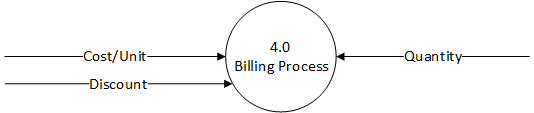
\includegraphics{Q1.png}

        \begin{choice}(1)
            \choice \answer{there is no output data flow from the process}
            \choice there are three data flow inputs to the process
            \choice there is no external entity
            \choice there is no data store
        \end{choice}
    \end{exercise}
    \begin{exercise}
        The following portion of a DFD is not correct as

        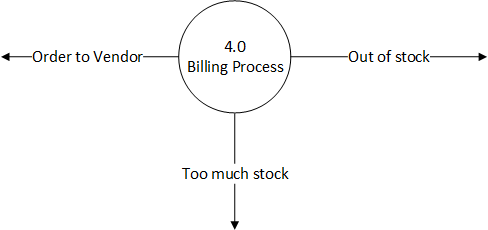
\includegraphics{Q2.png}
        \begin{choice}(1)
            \choice there are many data flows out of the process
            \choice \answer{there are no input data flows to the process}
            \choice the output does not go to an external entity
            \choice there is no data store
        \end{choice}
    \end{exercise}
    \begin{exercise}
        The following portion of DFD is wrong as

        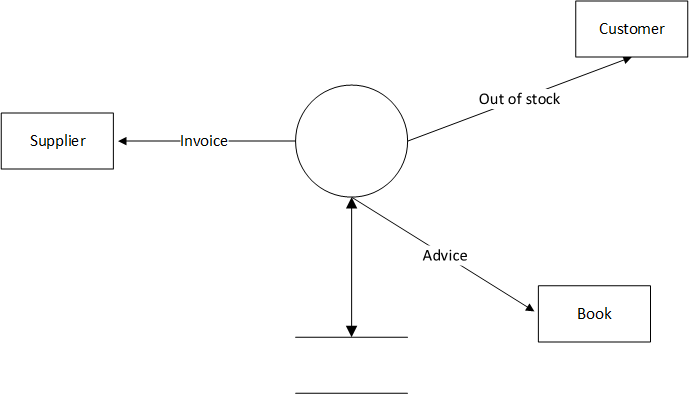
\includegraphics{Q3.png}
        \begin{choice}(1)
            \choice it has only one input
            \choice \answer{it writes and reads from the same data store}
            \choice the process name is missing
            \choice output data flows to two external entities
        \end{choice}
    \end{exercise}
    \begin{exercise}
        The following process diagram in a DFD is incorrect because

        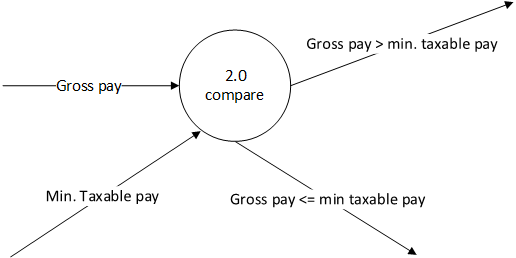
\includegraphics{Q4.png}
        \begin{choice}(1)
            \choice \answer{the process is a single decision}
            \choice the process is not specified correctly
            \choice there are too many input data flows
            \choice the process does not refer to a data store
        \end{choice}

    \end{exercise}
    \begin{exercise}
        The following portion of a DFD is incorrect because

        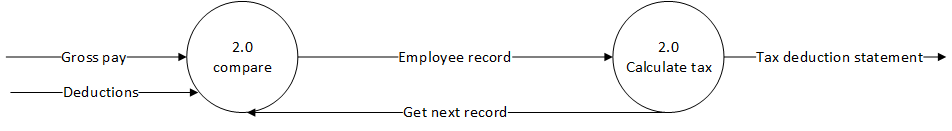
\includegraphics{Q5.png}
        \begin{choice}(1)
            \choice the processes do not refer to a data store
            \choice \answer{there is a loop between the two processes}
            \choice the processes are not specified correctly
            \choice this structure is disallowed in a DFD
        \end{choice}
    \end{exercise}
    \begin{exercise}
        Data flow in a DFD must have
        \begin{tasks}
            \task an arrow showing direction of flow of data
            \task a meaningful name
            \task a label such as: xyz
            \task no arrows as they are confusing
        \end{tasks}
        \begin{choice}(4)
            \choice (I) and (III)
            \choice (II) and (IV)
            \choice (III) and (IV)
            \choice \answer{(I) and (II)}
        \end{choice}
    \end{exercise}
    \begin{exercise}
        A context diagram \dots
        \begin{choice}(1)
            \choice describes the context of a system
            \choice  \answer{is a DFD which gives an overview of the system}
            \choice is a detailed description of a system
            \choice is not used in drawing a detailed DFD
        \end{choice}
    \end{exercise}
    \begin{exercise}
        A context diagram is used \dots
        \begin{choice}(1)
            \choice \answer{as the first step in developing a detailed DFD of a system}
            \choice in systems analysis of very complex systems
            \choice as an aid to system design
            \choice as an aid to programmers
        \end{choice}
    \end{exercise}
\end{questions}
\newpage
\section*{Answers}
\begin{multicols}{2}
    \getanswers
\end{multicols}
\end{document}